%!TeX root=MemoriaTFG.tex

\chapter{Tetris 99 and system built}

\section{Tetris version}
Tetris is a long running game series that has been ongoing since 1984, when Alexey Pajitnov invented it. Ever since it was created, many iterations of the game have been made, with each one of those somewhat altering the rules or adding new mechanics to spice things up. As previously mentioned, the project is being made under the Tetris 99 version, which implements the \ac{SRS}. This version has been chosen due to it being the most modern tetris up to date and because of the challenge of having our \ac{AI} work on another platform. 

\section{Game basics}
\begin{figure}[]
\centering
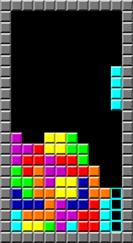
\includegraphics{image001}
\caption{\label{fig:gridExample}Tetris grid example}
\end{figure}

\begin{figure}[]
\centering
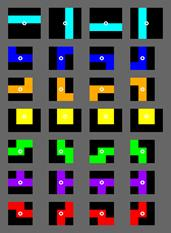
\includegraphics{image002}
\caption{\label{fig:pieces}Tetris pieces and their rotations}
\end{figure}

\begin{table}[h]
\begin{tabular}{
>{\columncolor[HTML]{F8F9FA}}l 
>{\columncolor[HTML]{F8F9FA}}l lll}
Single             & 100 × level difficulty   \\
Double             & 300 × level difficulty   \\
Triple             & 500 × level difficulty   \\
Tetris (Quadruple) & 800 × level difficulty 
\end{tabular}
\caption{\label{fig:scores}Tetris score by lines cleared}
\end{table}

\begin{table}[]
\begin{tabular}{
>{\columncolor[HTML]{F8F9FA}}l 
>{\columncolor[HTML]{F8F9FA}}l }
\hline
Combo       & 50 ×   combo count × level \\
Soft drop   & 1 per   cell               \\
Hard   drop & 2 per   cell              
\end{tabular}
\caption{\label{fig:scores2}Tetris score by movement and combos}
\end{table}

As many people already know, Tetris is a puzzle game consisting in trying to stack pieces up pieces and clear lines on a 10x20 grid. Whenever a line is filled to its maximum capacity it gets cleared and the blocks above it drop as many lines as were cleared. Whenever a piece is locked in place in an altitude higher than the game grid plus one you lose. A grid could look like figure~\ref{fig:gridExample}.

There is a total of 7 different pieces, each one of those having an associated colour that is usually maintained through all Tetris versions. Their names are I, J, L O, S, T and Z as seen in figure ~\ref{fig:pieces}.

As we can see in the image just referenced, each piece has four different orientations which can be accessed sequentially back and forth in the order shown, the small circle indicating the axis the piece rotates in.

The I and O pieces are a special case given that they do not use an actual block as their anchor point to rotate, making the first one shift one block up or down depending on the current position and the second one not rotate at all.

Now that we know their shapes, we see that the maximum number of lines that can be cleared at once is four. This is crucial because the score we obtain does not increase linearly, netting us higher scores the more lines we clear in one go.

The actual formula which dictates how many points we get can be seen in ~\ref{fig:scores}

More ways of obtaining points are soft drops (moving the piece down one cell), hard drops (letting the piece fall to the bottom) and combos (chaining line clears with different pieces), which go as \ref{fig:scores2}

Finally, there is T-spins, which is a mechanic that will be spoken about at the end of this block, once all the information surrounding the SRS has been laid out.
The scoring system just described works on single player game modes, but in Tetris 99, the main game mode actually involves 99 players concurrently battling against each other. Here line clears serve another purpose, sending “garbage lines” to the opponents. More on this system in the following section.


\section{UI and specifics}
\begin{figure}[]
\centering
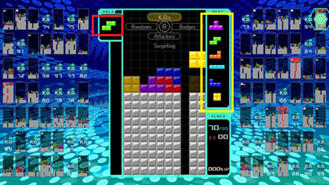
\includegraphics{image003}
\caption{\label{fig:tetris99game}Actual Tetris 99 game}
\end{figure}

An actual game of Tetris 99 will look like fig\ref{fig:tetris99game}.
There are many things that need to be analyzed to fully understand all the game aspects of this game version.

The first thing that should be mentioned is that we can see the upcoming 6 pieces that will have to be placed on the board (highlighted by the yellow square). Those are chosen from a bag containing all seven pieces, therefore making the game much more predictable as luck will not be impacting the game as much as with a fully random selector.

Then, there is the piece storage block (encapsulated by the red square), which allows us to save the current piece and draw the next one or, if there already is a stored one, to swap it out.

Last and more importantly, the background shows many more smaller Tetris boards, which belong to other players who are competing against you. In this mode you cannot see your score, and your performance is based on surviving the longest. When clearing lines, you now send garbage lines (grey blocks) to whoever of those players you are targeting:
\begin{itemize}
	\item	Clear two lines: Send one line of garbage
	\item	Clear three lines: Send two lines of garbage
	\item	Clear four lines: Send four lines of garbage
	\item	Clear the full board: +4 lines of garbage
\end{itemize}

Whenever you kill a player, a part of a badge is awarded to you. Each badge is increasingly more difficult to get, and you can only get up to four in total:
\begin{itemize}
   \item	Two knockouts: 25\% garbage bonus
   \item	Six knockouts:   50\% garbage bonus
   \item	14 knockouts:    75\% garbage bonus
   \item	30 knockouts:    100\% garbage bonus
\end{itemize}

It may seem quite difficult to complete all badges, but the method is eased by being able to steal the badges from a player you have defeated.
You can choose between five attacking modes to target different opponents:
\begin{itemize}
   \item	K.O.s: targets whoever is closer to losing the game.
   \item	Randoms.
   \item	Badges: targets whoever has more badges.
   \item	Attackers: targets whoever is attacking you.
   \item	Choice: manually select a specific player.
\end{itemize}

If you are targeted by multiple opponents, a boost to attack power is received:
\begin{itemize}
   \item	2 Opponents:	+1 Bonus lines sent
   \item	3 Opponents:	+3 Bonus lines sent
   \item	4 Opponents:	+5 Bonus lines sent
   \item	5 Opponents:	+7 Bonus lines sent
   \item	6+ Opponents:	+9 Bonus lines sent
\end{itemize}

This boost is applied before the badge attack boost.

It should also be noted that when receiving garbage lines, those will first be shown in the column right under your piece storage, and only be added to your board after some time. The time is indicated by 3 colour stages, being grey, yellow, and red, from best to worst. Garbage lines can also be cleared before they are added to your board by simply clearing lines.

\section{SRS (Standard rotation system)}
Now we can focus on the most intricate part of the game, the rotation system. The basics of this system have already been mentioned, however there is a much deeper pattern to it, which allows us to rotate pieces into places we would not normally be able to. These situations occur when a rotation that is not possible because a collision is detected, and the system tries to move the piece into four different offsets sequentially, sticking to whichever one works first. There are mainly two kinds of offsets, the ones that straight up ignore some collisions and allow you to rotate passing through blocks, and the ones that move you to another location. When an offset displaces you, it is known in game terms as a “kick”, and it should be noted that kicks can be performed against walls and pieces equally, propelling you in on or even two directions at the same time, even upwards. Because of the existence of upward kicks, a system limiting the number that can be performed had to be implemented to avoid infinite stalling.

As there is a very large variety of rotations and kicks that can be performed, only a few examples that represent most cases can be seen in figures \ref{fig:phase1}, \ref{fig:phase2}, \ref{fig:phase3}, \ref{fig:phase4}.

\begin{figure}
\centering
\begin{subfigure}{.4\textwidth}
  \centering
  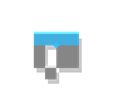
\includegraphics[width=.6\linewidth]{image004}
\end{subfigure}%
$\rightarrow$
\begin{subfigure}{.4\textwidth}
  \centering
  
\includegraphics[width=.6\linewidth]{image005}
\end{subfigure}
\caption{\label{fig:phase1}No kick phase}
\end{figure}

\begin{figure}
\centering
\begin{subfigure}{.3\textwidth}
  \centering
  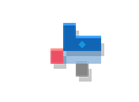
\includegraphics[width=.8\linewidth]{image006}
\end{subfigure}%
$\rightarrow$
\begin{subfigure}{.3\textwidth}
  \centering
  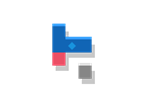
\includegraphics[width=.8\linewidth]{image007}
\end{subfigure}%
$\rightarrow$
\begin{subfigure}{.3\textwidth}
  \centering
  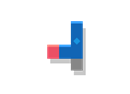
\includegraphics[width=.8\linewidth]{image008}
\end{subfigure}
\caption{\label{fig:phase2}Right kick phase}
\end{figure}

\begin{figure}
\centering
\begin{subfigure}{.3\textwidth}
  \centering
  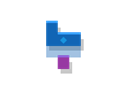
\includegraphics[width=.8\linewidth]{image009}
\end{subfigure}%
$\rightarrow$
\begin{subfigure}{.3\textwidth}
  \centering
  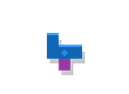
\includegraphics[width=.8\linewidth]{image010}
\end{subfigure}%
$\rightarrow$
\begin{subfigure}{.3\textwidth}
  \centering
  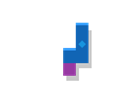
\includegraphics[width=.8\linewidth]{image011}
\end{subfigure}
\caption{\label{fig:phase3}Up right kick phase}
\end{figure}

\begin{figure}
\centering
\begin{subfigure}{.4\textwidth}
  \centering
  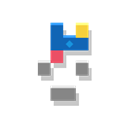
\includegraphics[width=.6\linewidth]{image012}
\end{subfigure}%
$\rightarrow$
\begin{subfigure}{.4\textwidth}
  \centering
  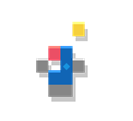
\includegraphics[width=.6\linewidth]{image013}
\end{subfigure}
\caption{\label{fig:phase4}Down kick phase}
\end{figure}

Now that we have showed some examples, we can talk about T-spins. As its own name implies T-spins are performed using the T piece, and they happen whenever we manage to offset the piece into clearing 1, 2 or three lines, giving us 2, 4 and 6 garbage lines/800 × level, 1200 × level, 1600 × level respectively.

\begin{figure}[h]
\centering
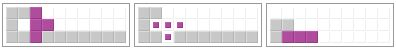
\includegraphics{image014}
\caption{\label{fig:tspin1}T-spin single}
\end{figure}

\begin{figure}
\centering
\begin{subfigure}{.33\textwidth}
  \centering
  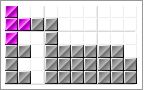
\includegraphics[width=.8\linewidth]{image015}
\end{subfigure}%
\begin{subfigure}{.33\textwidth}
  \centering
  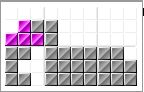
\includegraphics[width=.8\linewidth]{image016}
\end{subfigure}%
\begin{subfigure}{.33\textwidth}
  \centering
  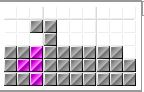
\includegraphics[width=.8\linewidth]{image017}
\end{subfigure}
\caption{\label{fig:tspin2}T-spin double}
\end{figure}

\begin{figure}[h]
\centering
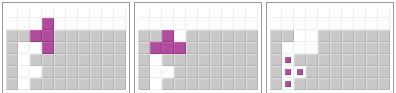
\includegraphics{image018}
\caption{\label{fig:tspin3}T-spin triple}
\end{figure}


\section{Our system}
Having defined all important aspects of tetris 99, an environment similar enough had to be built in order for the \ac{AI} not to find itself in a foreign situation when being tested in the Nintendo Switch. Thus a search for similar looking tetris implementations had to be done. Unfortunately, as mentioned when talking about the project setbacks, no complete candidates where found.

Thanks to the information found regarding how the \ac{SRS} works and a project giving an example implementation in C\#, we built from scratch a similar looking system that fulfilled our requirements. The system is constituted by three classes, board, piece and tile, each one being controlled and used by the one mentioned before it. Finally, the the script called "tetris.py" unites all of them together and creates a visual interface to play on and show the net's output whenever requested.

To explain the following data structure a bottom up approach will be used in order to follow the thought process behind its implementation.

\subsection{Tile}
Tile is a class very short class containing a position in two dimensions (x,y) and a colour in rgb format. It also includes a method that given a center point and a direction, rotates its own coordinates once.

\subsection{Piece}
A piece object is consituted by "n" number of tiles depending on the piece type. There is a piece child class for each possible piece type and every one of them contains a list of each of the displacements or kicks that can be performed given a rotation. The method rotate piece loops through each tile calling their own rotate method using the center tile as the anchor.

\subsection{Board}
Board is the biggest class of the three consituting the data structure. It is in charge of implementing all the tetris 99 rules there are. Here there is also a piece rotating method, which is in charge of checking wether a kick can be performed or not, given it has the position of each of the blocks and the walls. Despite having implemented the t-spin moves a system that puntuates them has not been built, as it will not be used to reward the neural net (more information on that in the neural net section). 

\subsection{Tetris game}
Finally, we have the tetris script, coded using pygame. There is two different implementations within it which will be used to our convenience. The first one calls the main game loop and allows us to play the game normally, reading our keyboard input and calling the appropiate board methods to perfrom each one of them:

\begin{itemize}
   \item	$\downarrow$: "Soft drop", drops the piece down by one line.
   \item	$\uparrow$: "Hard drop", drop the piece as far down as it can.
   \item	$\leftarrow$: Moves left by one column if possible.
   \item	$\rightarrow$: Moves right by one column if possible. 
   \item	space bar: Stores the current piece if a piece was not just stored.
   \item	"a": Rotates left.
   \item	"d": Rotates right.
\end{itemize}

The second one is used by the neural net to show each of its moves. This means that the board game object is manipulated solely by the AI and the scrpit is only used to render the visual information of it by calling the applicable methods.

Either way, both can be stopped by exiting the window clicking the top right "X".
